\documentclass[12pt]{article}
\usepackage{amssymb}
\usepackage[UTF8]{ctex}
\usepackage{geometry}
\usepackage{units}
\usepackage{pifont}
\geometry{
	a4paper,
	total={150mm,237mm},
	left=30mm,
	top=27mm,
	}
\usepackage{amsmath}
\usepackage{enumerate}
\usepackage{lipsum}
\usepackage{graphicx}
\usepackage{hyperref}
\usepackage{indentfirst}
\usepackage[graphicx]{realboxes}
\usepackage{booktabs}
\usepackage{cases}
\usepackage{subfig}  
\usepackage{float}
\usepackage{xcolor}
\setlength{\parindent}{2em}
\title{Lab6}
\author{姓名:陈锐林,学号:21307130148}
\date{\today}

\begin{document}
\maketitle
\begin{large}
    \noindent 实验1\\
\end{large}
一、实验思路\par
1.这题思路比较简单,首先要完善对NDIRECT、NINDIRECT的定义和进行inode,dinode的修改;主要是为了和目标中扩展一个块作对应。其中NINDIRECT应该是(BSIZE/sizeof(uint)),也就是要求的1024/4=256;还要记得修改MAXFILE的定义,改为
NDIRECT + NINDIRECT + NINDIRECT * NINDIRECT。\par
2.接着主要是完善bmap函数,参考已有的bmap,能看出要用以下函数:balloc用于分配,bread进入目录,log\_write进行写log,以及最后brelse先前bread的目录。接着参照对于但间接数据块的流程,完善两级的。首先加载NDIRECT+1的块(如果未分配要补上),接着记载目录进入下一级;
未分配还要补上;最后才进入二级,并重复操作。其中三次取的索引就应该是:NDIRECT+1,bn / NINDIRECT,bn\% NINDIRECT。\par
3.最后是在itrunc函数中完善释放块的任务。可以看到很类似的,对于1级的,就是进入目录一一释放;那么2级的就是在1级的基础上,先不释放1级,再依次遍历2级数据并释放。\par

\noindent 二、具体实现\par
1.完成预定义:NDIRECT,NINDIRECT,MAXFILE的定义如下,为了对应缩小了1的NDIRECT,将inode,dinode中的addrs改为"addrs[NDIRECT + 2]"(未展示).
\begin{figure}[H]
    \centering
    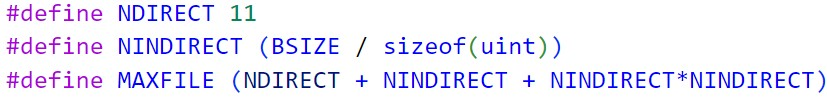
\includegraphics[width=0.8\textwidth]{lab6-1.jpg}
\end{figure}\par
2.bmap函数:仿照前面的1级处理,完善"实验思路2."的bmap函数。根据文件系统的索引规则,确定两次读取的内容bp1和bp2;未分配时及时分配即可。
\newpage
\begin{figure}[H]
    \centering
    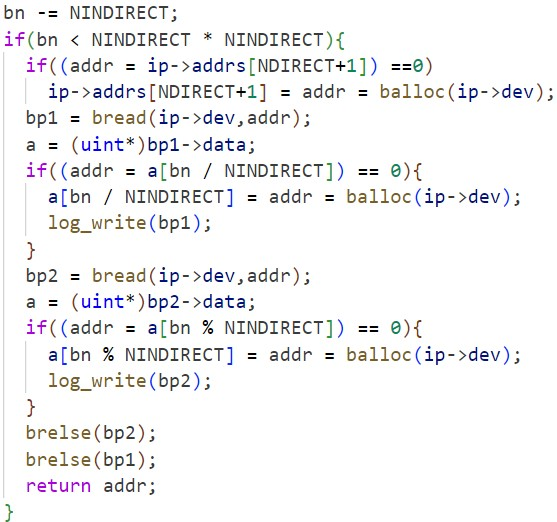
\includegraphics[width=0.7\textwidth]{lab6-2.jpg}
\end{figure}\par
3.itrunc函数:完善释放的函数,当ip-addr指向2级的块是进入处理。内部使用两个for循环进行递归,凡是分配了的都要及时bfree;最后每次退出要及时brelse;最外部完成对直接数据块的释放。
\begin{figure}[H]
    \centering
    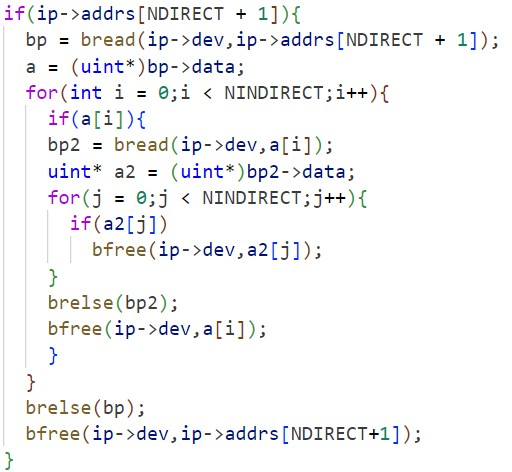
\includegraphics[width=0.7\textwidth]{lab6-3.jpg}
\end{figure}\par
\newpage
\begin{large}
    \noindent 实验2\\
\end{large}
一、实验思路:\par
1.准备工作,包括:(1)系统调用老生常谈的user/usys.pl、user/user.h、kernel/syscal.h、kernel/syscal.c,不再赘述;(2)kernel/stat.h中添加新的文件类型T\_SYMLINK,为4(顺延);(3)kernel/fcntl.h中添加新标志O\_NOFOLLOW,考虑到传递给open时使用or操作,所以必须是独立的;顺延下取0x800。\par
2.这里打算直接在sysfile.c里实现symlink,就不设空了。参考sysfile其他函数和xv6的资料,能看到,开始/结束文件系统操作需要调用函数nameiparent()获取父目录信息,begin\_op()和end\_op(),ilock()用于锁定inode,ialloc()用于分配inode,writei()用于向inode写入链接信息,dirlink()用于在父目录建立链接,iupdate()用于更新inode,以及完成操作后应该要用iunlockput()释放锁并增加计数,用
iput()增加计数。所以symlink的过程应该是这样的:通过argstr获得目标路径和链接路径;nameiparent获取目标路径的父目录和链接名称: ialloc分配一个inode并writei写入目标路径;dirlink链接到父目录;最后更新连接数。\par
3.更改open函数。根据已有的模板,主要是多添一条,在ip->type == T\_SYMLINK \&\& omode != O\_NOFOLLOW)时进入该处理。之后我们应该打开链接的地址;考虑到多次链接的情况,需要包装一个循环解决这个问题,循环终止条件就是(1)有循环链接(简单标识为寻找次数大于12)或者(2)不再是T\_SYMLINK类型了。具体的实现
利用readi函数读取当前inode对应目标路径和namei获取新的inode。while(...){readi(...),namei(...)}。\\
二、具体实现\par
1.此处省略。\par
2.(1)读取参数;(2)获得父目录信息;(3)分配一个inode并写入目标路径:
\begin{figure*}[!h]
    \centering
    \subfloat[读参数]{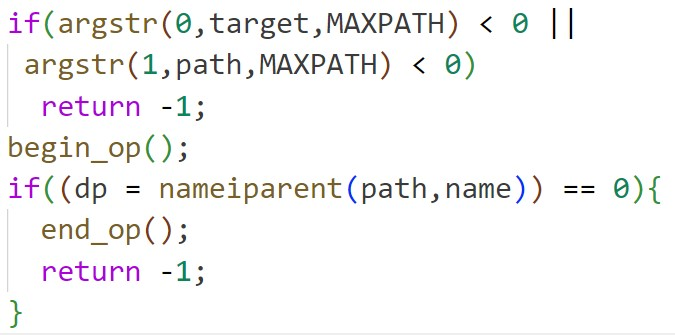
\includegraphics[width=0.48\textwidth]{lab6-4.jpg} \label{X}}
    \hfill
    \subfloat[得父目录信息]{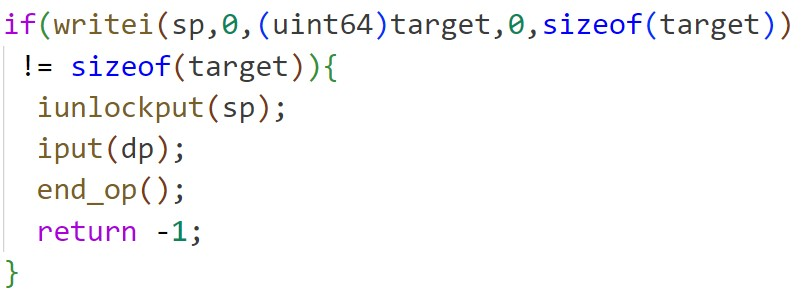
\includegraphics[width=0.48\textwidth]{lab6-5.jpg} \label{Y}}
\end{figure*}\par
(3)链接到父目录;(4)完成计数更新。注:begin\_op()和ilock()等因为篇幅原因没有放入。
\newpage
\begin{figure*}[!h]
    \centering
    \subfloat[读参数]{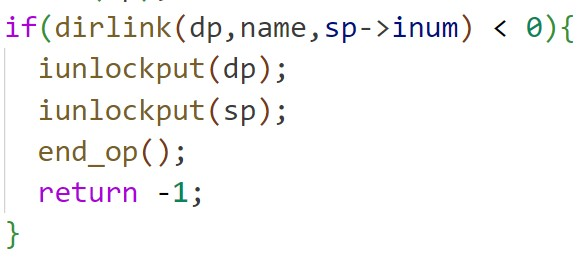
\includegraphics[width=0.48\textwidth]{lab6-6.jpg} \label{X}}
    \hfill
    \subfloat[得父目录信息]{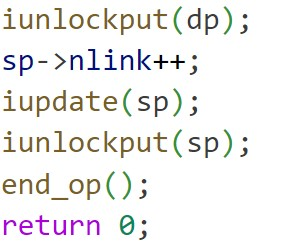
\includegraphics[width=0.2\textwidth]{lab6-7.jpg} \label{Y}}
\end{figure*}\par
3.修改open函数,(1)open函数中特判如下,symlink\_ip函数是包装出去实现的:
\begin{figure}[H]
    \centering
    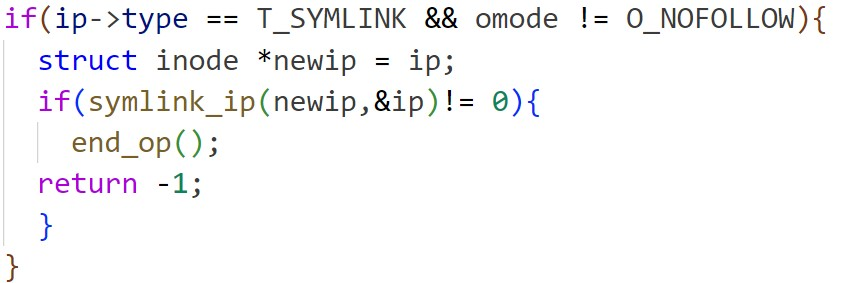
\includegraphics[width=0.5\textwidth]{lab6-8.jpg}
\end{figure}\par
(2)symlink\_ip函数中,主体循环如下。主要是如上利用了readi读取当前inode的目标路径和namei获取新的inode。
\begin{figure}[H]
    \centering
    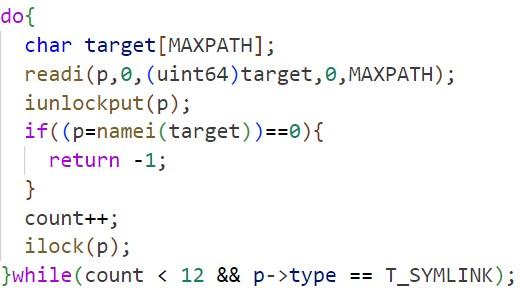
\includegraphics[width=0.6\textwidth]{lab6-10.jpg}
\end{figure}
\begin{large}
    \noindent $\bigstar $测试结果(make grade后的结果,两个实验一起的)
\end{large}
\begin{figure}[H]
    \centering
    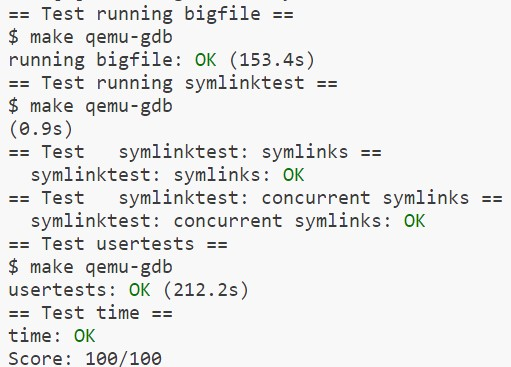
\includegraphics[width=0.6\textwidth]{lab6-9.jpg}
\end{figure}
\end{document}